% 2016 年全国卷Ⅱ文科第 22 题：正方形内的垂足及连线
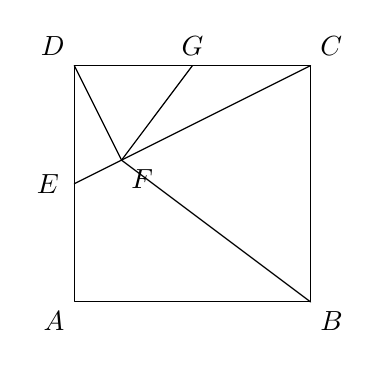
\begin{tikzpicture}[line width=0.45pt, line cap=round, line join=round]
  \coordinate (A) at (0,0);
  \coordinate (B) at (3,0);
  \coordinate (C) at (3,3);
  \coordinate (D) at (0,3);
  \coordinate (E) at (0,1.5);
  \coordinate (G) at (1.5,3);
  \coordinate (F) at (0.6,1.8);

  \draw (A) -- (B) -- (C) -- (D) -- cycle;
  \draw (C) -- (E);
  \draw (D) -- (F);
  \draw (B) -- (F);
  \draw (G) -- (F);

  \node[below left] at (A) {$A$};
  \node[below right] at (B) {$B$};
  \node[above right] at (C) {$C$};
  \node[above left] at (D) {$D$};
  \node[left=2pt] at (E) {$E$};
  \node[above] at (G) {$G$};
  \node[below right] at (F) {$F$};
\end{tikzpicture}
